% !TEX root = ../thesis.tex

\chapter{Context}
\label{chap:context}

\cleanchapterquote{No computer has ever been designed that is ever aware of what it's doing; but most of the time, we aren't either.}{Marvin Minsky}{(Father of the field of AI)}


% ------------------------------------------------------------------------------

In our journey to separation of form and content in neural networks, we will now go through the stepping stones that led to \citeauthor{Gatys2015B}'s Neural Style algorithm: 1) advances in object recognition using deep neural networks, 2) the development of techniques for visualizing intermediate processing steps within deep neural networks, and 3) the evolution of style transfer tasks.

In Chapter~\ref{chap:theory} we introduced convolutional neural networks (CNNs) and gave a glimpse of how they can be used for image recognition tasks.
In this chapter, we will describe, in detail, the challenges in object recognition and how CNNs, traditionally outperformed by other techniques, have become the state of the art.
Interestingly, it is not so well understood how some network architectures are better than others and, therefore, how current ones can be improved.
Also in this chapter, we will see a number of visualization techniques that have been recently developed with the intention of eliciting new intuitions to help us move forward in the field of neural networks, some of them with unexpectedly appealing results.
Considerations on their potential artistic implications quickly appeared, and so this chapter also covers an introduction to artistic rendering and a few influential style transfer techniques.


% ------------------------------------------------------------------------------

\section{Object Recognition}
\label{sec:context:object-recognition}

We refer to the task of general object recognition as recognizing any object in natural images and it has been a very difficult problem to solve until recently.
In \autoref{fig:sec:context:object-recognition} we can see a typical task of general object recognition on a natural image.
\citet{Pinto2008} concluded in 2008 that the difficulty of the task stems from the fact that any 3D object in the world has an infinite number of representations in 2D images, as position, pose, lighting, and background vary with respect to the observer.
At the same time, as we argued in Chapter~\ref{chap:intro}, the brain is able to perform general object recognition in the real world without any apparent struggle, and so replicating the human visual system started to be perceived as a possible strategy to fully capture the complexity of the task.

\begin{figure}[t]
  \begin{subfigure}[b]{0.5\textwidth}
    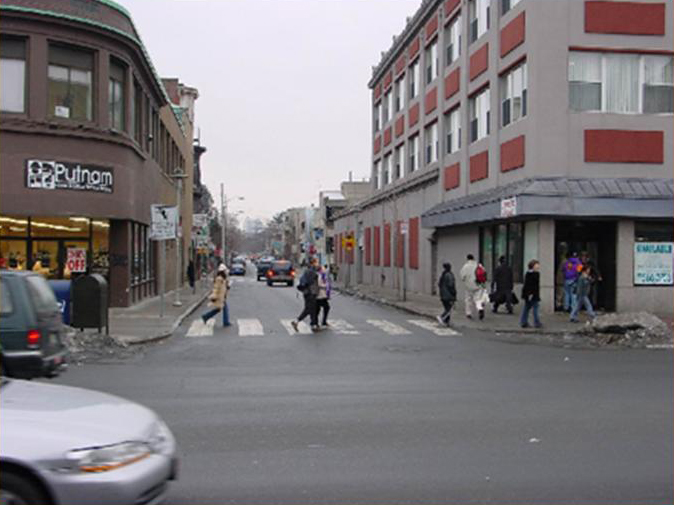
\includegraphics[width=\textwidth]{gfx/object-recognition-1}
    \label{fig:sec:context:object-recognition-1}
  \end{subfigure}
  \hfill
  \begin{subfigure}[b]{0.5\textwidth}
    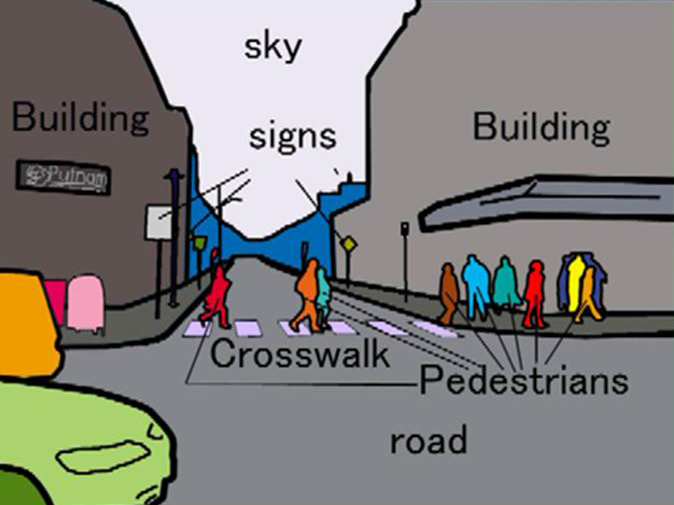
\includegraphics[width=\textwidth]{gfx/object-recognition-2}
    \label{fig:sec:context:object-recognition-2}
  \end{subfigure}
  \caption{
    Typical object recognition task \cite{Wolf}.
    Object recognition consists of locating objects on a natural image and giving them correct labels.
  }
  \label{fig:sec:context:object-recognition}
\end{figure}

As we mentioned in Chapter~\ref{chap:theory}, CNNs successfully emulate biological visual systems.
\citeauthor{LeCun2004B} in \cite{LeCun2004B} had already compared CNNs in 2004 with traditional techniques such as K-Nearest Neighbors and Support Vector Machines (SVM) for small-scale object recognition, finding that CNNs obtained better results in general and, especially, in non-normalized conditions.
\citeauthor{LeCun2004B} used the NORB dataset for training, being at that time the largest available one, with 97200 pre-processed image pairs of 50 different objects of 5 categories.

\citeauthor{Pinto2008} also argued NORB and other datasets available at that time, in the order of tens of thousands of images, such as Caltech-101/256 \cite{Fei-Fei2007,Griffin2007} or CIFAR-10/100 \cite{Krizhevsky2009}, were not large nor diverse enough to be used for general object recognition training.
They found systems trained with them were highly susceptible to the variations described above in this section (i.e. pose, position, lighting, etc.) and claimed that, for a learning system to be robust against them, it would need to capture the essence of the domain rather than rely on trivial regularities of the training samples.
Such a dataset, one that could consistently represent the domain (i.e. all the object in the real world without with all their variance), would not only required to be much larger than those available back in 2008 but also to contain unbiasedly-selected natural images.

Being clear the need for larger datasets at that point, ImageNet \cite{Deng2009} was handcrafted via crowdsourcing with the aim of organizing a fraction of the vast number of images on the Internet and making them available for object recognition tasks.
ImageNet is a large-scale, comprehensive, and diverse dataset of 15 million high-resolution accurately-labeled images, organized in a semantic hierarchy of 22000 categories.
In it, each noun in English, coming from the lexical database WordNet \cite{Wilkniss1998}, is associated with hundreds of clean images.
The achievements of ImageNet are two-fold.
On the one hand, the images depict representations of the words under many different perspectives and lighting conditions, allowing robustness against visual variability.
On the other hand, the hierarchical structure of the dataset makes it possible to interlink concepts, allowing algorithms to recognize several concepts at the same time (e.g. dog, therefore mammal and animal as well).

Based on the ImageNet dataset, the ImageNet Large-Scale Visual Recognition Challenge (ILSVRC) has established itself as the de-facto benchmark for object recognition algorithms.
Run as a yearly competition since 2010, it has triggered some of the most important advances in the field \cite{Russakovsky2015}.
Deep neural networks did not enter the scene until 2012.
CNNs had been terribly expensive to apply in large scale to high-resolution images until then, but \citet{Krizhevsky2012} finally managed to train a sufficiently large network for ILSVRC leveraging multiple GPUs.
They run a GPU-optimized implementation of 2D convolutional neural networks and used ImageNet as their training set, which was diverse enough to prevent severe overfitting.

The relevance of deep neural networks in object recognition tasks did nothing but increase in the last few years, as they keep getting the top scores each year at ILSVRC \cite{Russakovsky2015}.
At the time of writing this thesis, the use of GPU computing in deep neural networks is now generalized, facilitated by deep learning frameworks implementing GPU-optimized implementations of convolutions and all the necessary operations both for classification and training \cite{Bahrampour2015}.
Deep learning frameworks are just programming libraries that provide out-of-the-box tools for easily implementing deep neural networks, allowing researchers to focus on the architecture.
Some of the most popular ones currently are Caffe, developed by the Berkeley Vision and Learning Center \cite{Jia2014}; Theano, developed by l’Université de Montréal \cite{Bergstra2010}; TensorFlow, developed by Google \cite{Abadi2015}; or Torch, supported by Facebook and Nvidia \cite{Collobert2002}.

Deep learning frameworks have helped much to the reproducibility of experiments with neural networks, as they simplify the requirements for sharing architectures as well as trained models between researchers.
In Chapter~\ref{chap:system} we will see how the VGG network \cite{Simonyan2014}, one of the winners of ILSVRC 2014, rivaling human performance \cite{Russakovsky2015}, implemented in Caffe, and publicly available \cite{Simonyan2014web}, is used to effectively separate style and content.
Next, we will talk about the interest that grew for understanding what exactly happens within intermediate layers of CNNs trained for object recognition, resulting in a number of visualization techniques with surprising results.


% ------------------------------------------------------------------------------

\section{Visualization of Convolutional Neural Networks}
\label{sec:context:deep-visualization}

For a long time, neural networks have been perceived as ``black boxes''.
Although we can perceive the training phase as a simple function optimization process, trained models consist of a large number of trained non-linear parameters that we cannot easily comprehend in a sensible way \cite{Yosinski2015}.
Deep neural networks, like CNNs, are particularly difficult to study due to their size.
Learnable parameters in them are in the order of millions and this makes us understand very little about why some models work better than others.
Gaining insight into how trained models function is one way towards improving them, as new intuitions may arise or wrong assumptions may become apparent.

In an effort to shed some light, several studies have been done lately in the direction of providing techniques for visualizing different representations of what happens within CNNs trained for object recognition \cite{Dosovitskiy2015,Yosinski2015,Zeiler2014}.
We know each layer of trained CNNs extracts increasingly higher-level features of an input image until eventually, the last layer emits a decision of what was depicted in the image.
As we described in \autoref{sub:concepts:convnets:properties}, lower layers tend to extract edges or corners, while intermediate ones look for more complex elements like shapes, faces, or textures.
Finally, the last few layers use them to interpret high-level concepts like forests or streets.
Some of the visualization techniques we are about to see help us inspect how this actually happens.

\citet{Mahendran2014} study how to obtain different visualizations from the internal representations at intermediate CNN layers showing that, as expected, CNNs gradually build an increasing amount of tolerance towards variance.
This is visible in \autoref{fig:sec:context:deep-visualization:deep-visualization-reconstructions-1}, as representations of the initial monkey image become fuzzier, less specific layer after layer.
For constructing these visualizations, \citeauthor{Mahendran2014} use gradient descent to find a new image that matches the feature space at a particular layer in a very similar way as we will discuss in more detail in Chapter~\ref{chap:system}.
Interestingly, selecting different subsets of feature channels produces texturized versions of the original image, as shown in \autoref{fig:sec:context:deep-visualization:deep-visualization-reconstructions-2}.

\begin{figure}[b]
  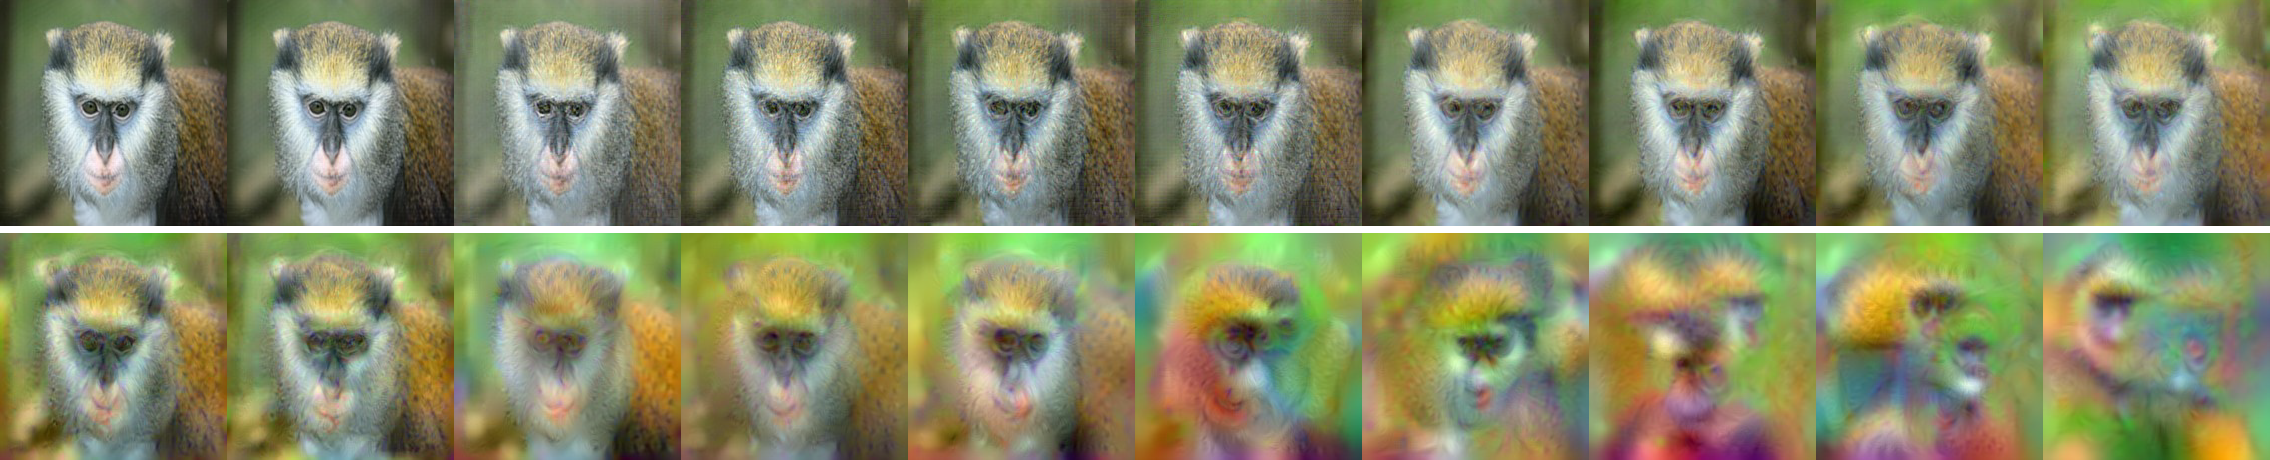
\includegraphics[width=\textwidth]{gfx/deep-visualization-reconstructions-1}
  \caption{
    CNN layer visualizations of a monkey image generated via gradient descent \cite{Mahendran2014}.
    Whereas the first layers (top row) maintain faithful representations of the original image, although increasingly fuzzy, invariance seems be appear in the last few ones (bottom row).
  }
  \label{fig:sec:context:deep-visualization:deep-visualization-reconstructions-1}
\end{figure}

\begin{figure}[t]
  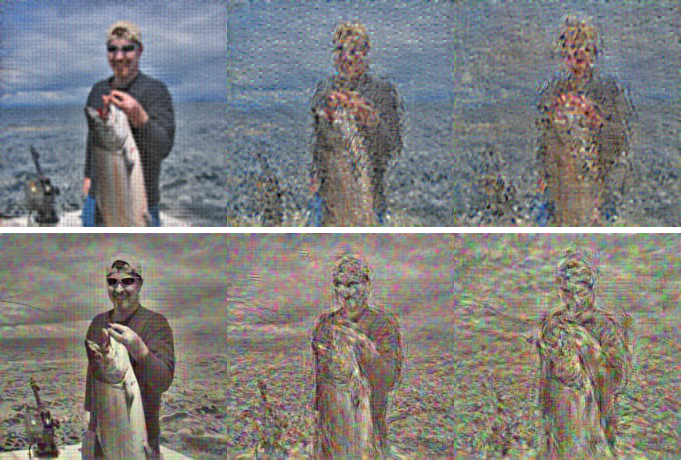
\includegraphics[width=\textwidth]{gfx/deep-visualization-reconstructions-2}
  \caption{
    CNN visualization of the first convolutional layer selecting different subsets of feature channels for the gradient descent generation \cite{Mahendran2014}.
    Depending on the selected channels, the visualizations are tuned towards different image parameters, producing texturized versions of the original image.
  }
  \label{fig:sec:context:deep-visualization:deep-visualization-reconstructions-2}
\end{figure}

\citet{Simonyan2014B} propose another visualization method, also through gradient descent, that generates class notions from a trained CNN.
That means a new image is generated in a way that the trained CNN would classify it with total certainty as the desired object.
In \autoref{fig:sec:context:deep-visualization-class}, some examples of this technique are displayed with clearly psychedelic results.
The generated images do not resemble natural images very much, more like graphic artifacts instead, but the network will anyway classify them correctly as these artifacts have been generated to cause precisely the right neural activations.

\begin{figure}[t]
  \begin{subfigure}[b]{0.3\textwidth}
    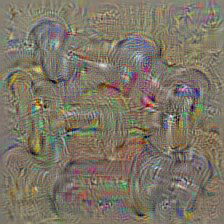
\includegraphics[width=\textwidth]{gfx/deep-visualization-class-1}
    \caption{dumbbell}
    \label{fig:sec:context:deep-visualization-class-1}
  \end{subfigure}
  \hfill
  \begin{subfigure}[b]{0.3\textwidth}
    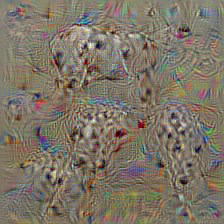
\includegraphics[width=\textwidth]{gfx/deep-visualization-class-2}
    \caption{dalmatian}
    \label{fig:sec:context:deep-visualization-class-2}
  \end{subfigure}
  \hfill
  \begin{subfigure}[b]{0.3\textwidth}
    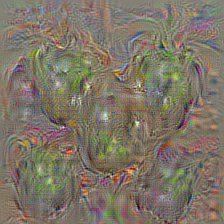
\includegraphics[width=\textwidth]{gfx/deep-visualization-class-3}
    \caption{bell pepper}
    \label{fig:sec:context:deep-visualization-class-3}
  \end{subfigure}
  \par\medskip
  \begin{subfigure}[b]{0.3\textwidth}
    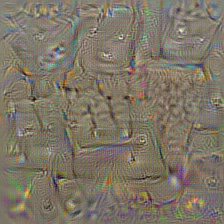
\includegraphics[width=\textwidth]{gfx/deep-visualization-class-4}
    \caption{keyboard}
    \label{fig:sec:context:deep-visualization-class-4}
  \end{subfigure}
  \hfill
  \begin{subfigure}[b]{0.3\textwidth}
    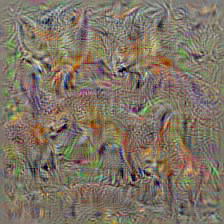
\includegraphics[width=\textwidth]{gfx/deep-visualization-class-5}
    \caption{kit fox}
    \label{fig:sec:context:deep-visualization-class-5}
  \end{subfigure}
  \hfill
  \begin{subfigure}[b]{0.3\textwidth}
    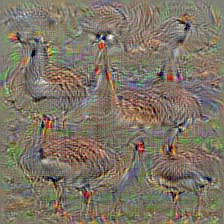
\includegraphics[width=\textwidth]{gfx/deep-visualization-class-6}
    \caption{goose}
    \label{fig:sec:context:deep-visualization-class-6}
  \end{subfigure}
  \caption{
    Images generated with gradient descent to artificially generate a desired classification, given a trained CNN \cite{Simonyan2014B}.
  }
  \label{fig:sec:context:deep-visualization-class}
\end{figure}

Google's DeepDream algorithm \cite{Mordvintsev2015} uses this same visualization technique to produce dream-like images in a process they call ``inceptionism'', useful for getting an idea of the level of abstraction a particular layer has achieved in its understanding of images.
DeepDream works as some sort of glorified \emph{pareidolia} that enhances whatever a trained CNN recognizes in an original image, replicating it in different sizes on every pass.
\autoref{fig:sec:context:deep-visualization:dream-buildings} shows images depicting scenery produced by DeepDream using random noise images as input and a CNN trained on places as the dreamer.
It can be explained because the a CNN trained on recognizing places has probably seen lots of structures, fountains and trees.
Also, because white noise images carry no information, we could say that these images are purely a product of the neural network's understanding of the world.

\begin{figure}[p]
  \begin{subfigure}[b]{\textwidth}
    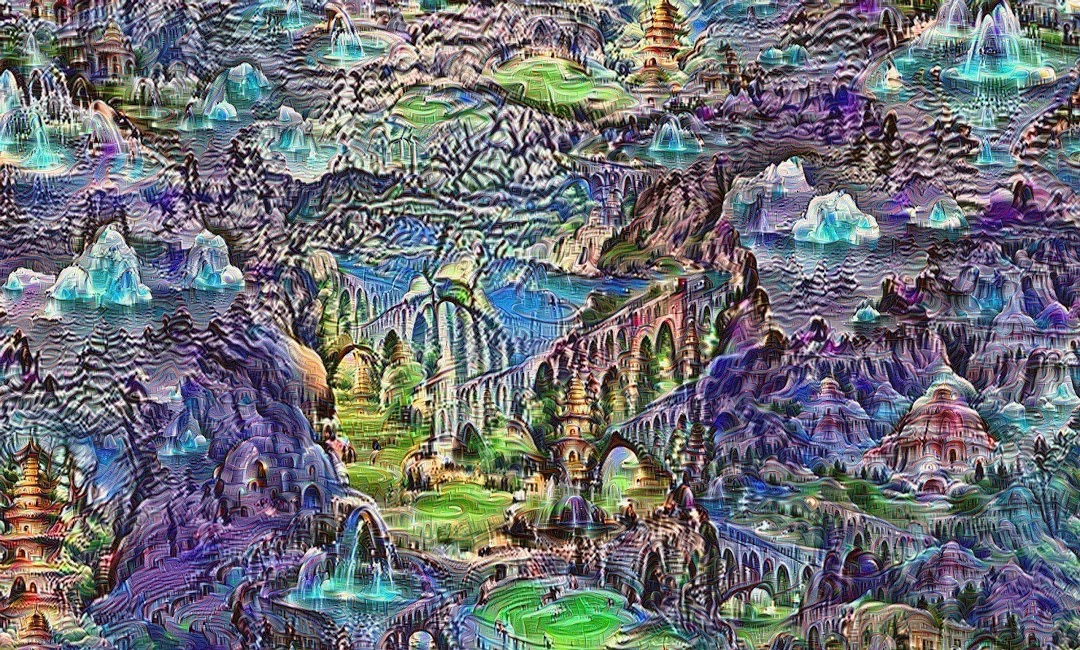
\includegraphics[width=\textwidth]{gfx/dream-buildings-1}
  \end{subfigure}
  \par\medskip
  \begin{subfigure}[b]{\textwidth}
    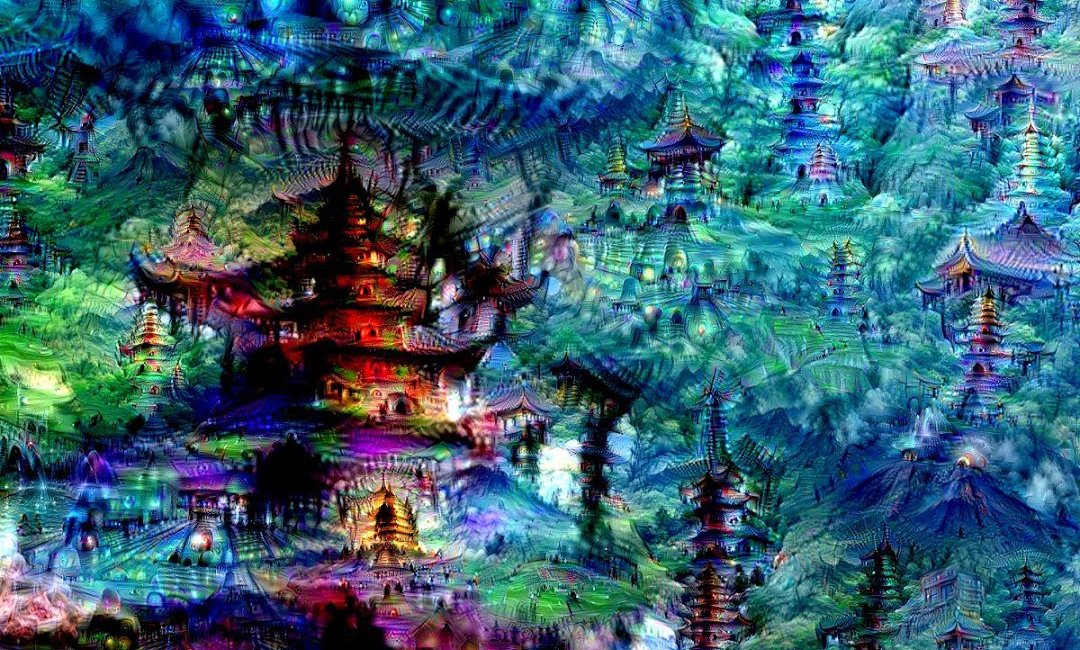
\includegraphics[width=\textwidth]{gfx/dream-buildings-2}
  \end{subfigure}
  \caption{
    Images generated with DeepDream from a white noise image and a CNN trained on places by the MIT Computer Science and AI Laboratory \cite{Mordvintsev2015}.
    Pagodas, fountains, bridges, and trees seem to be the most recurrent elements on them because the CNN was trained with thousand of images of them.
    Therefore, when ``dreaming,'' that is what the network sees.
  }
  \label{fig:sec:context:deep-visualization:dream-buildings}
\end{figure}

One final example of visualizations is given by \citet{Nguyen2014}, highlighting some of the problems of current CNN models.
Although they already rival human performance in many aspects, we can easily fool them by generated images that, by no means, resemble anything of what they claim to recognize.
For instance, in \autoref{fig:sec:context:deep-visualization:deep-visualization-fooling} we observe some of these fooling images that CNNs classify with total certainty as belonging to the categories shown below them.
These images have been generated with an evolutionary algorithm that applies random modifications and keeps those that better fit the desired category.

\begin{figure}[t]
  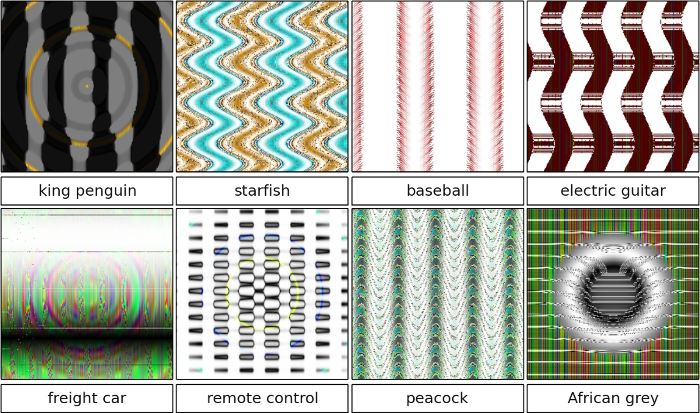
\includegraphics[width=\textwidth]{gfx/deep-visualization-fooling}
  \caption{
    Mislabeled images by a CNN trained for object recognition \cite{Nguyen2014}.
    Called ``fooling images'' and obtained with an evolutionary algorithm that applies random perturbations (mutation and/or crossover) on images and keeps those that produce the highest prediction in a desired category.
  }
  \label{fig:sec:context:deep-visualization:deep-visualization-fooling}
\end{figure}

All visualization methods described above hold some degree of artistic ``intention,'' as their respective authors observe.
First, \citeauthor{Mahendran2014}'s texturized images in \autoref{fig:sec:context:deep-visualization:deep-visualization-reconstructions-2} emerge naturally without the trained network having been encouraged to show it in any way.
Then, \citeauthor{Mordvintsev2015} speculate about the artistic implications of DeepDream, both as a rendering tool and as a step towards understanding the essence of the creative process in the human brain.
Lastly, \citeauthor{Nguyen2014} submitted some of these images to a selective art contest, the \emph{University of Wyoming 40th Annual Juried Student Exhibition}, got a third of them accepted, and some of them even received an award.

Artistic rendering, however, has been traditionally studied as a field of computer vision, and the problem of the separation of style and content was identified long ago as one of the main challenges for applying \emph{style transfer}.


% ------------------------------------------------------------------------------

\section{Style Transfer}
\label{sec:context:style-transfer}

We can understand artworks and paintings as the composition of form and content, as we commented in Chapter~\ref{chap:intro}.
Style transfer is the task of synthesizing a new stylized image with the same content as some source image and the style of a style sample.
To accomplish style transfer, not only the style-content combination is important, but even more so is the definition and extraction of style and content.
The difficulty of the latter is intrinsic to the separation of style and content, which is a very fundamental problem, since not even in the history of art literature seems to be a consensus as to what is content and what is style \cite{Xie2007}.

Because of this fundamental difficulty, we cannot use any formally-described evaluation for style transfer, and so we resort to appealing the human visual system as it will be the ultimate consumer of the generated images \cite{Lin2011}.
The main criteria commonly used are the score from an \emph{artistic Turing test} and the \emph{perceptual quality}.
Whereas the artistic Turing test score will be higher the more difficult it is for humans to distinguish generated images from those created by hand \cite{Kyprianidis2013}, the perceptual quality refers to the subjective degree of similarity with the original images providing content and style.

Style transfer is studied in the field of \emph{non-photorealistic rendering}, in development since the late 1980s as a branch of computer vision, which attempts to provide tools for mimicking the style of paintings or animated cartoons in digital art, both in 2D and 3D \cite{Lee2010, Kyprianidis2013}.
Non-photorealistic rendering has become a highly multidisciplinary field, being influenced by progress done in computer graphics, perceptual modeling, and human-computer interaction.
We will focus only on small collection of 2D image-based style transfer techniques.
In particular, we will analyze those based on texture synthesis most closely related to Neural Style \cite{Gatys2015B}.

Style transfer is often approached as a texture transfer operation, sharing many of the challenges of texture synthesis \cite{Ashikhmin2003}.
Given a small texture example, texture synthesis algorithms try to generate a texture of arbitrary size.
On the other hand, texture transfer takes a target image and a texture source and modifies part of the target image with information with the given texture, while trying to maximize the perceptual quality of the result.

\citet{Hertzmann2001} proposed in 2001 a statistical-based method for style transfer called Image Analogies.
It generates a new image $B'$ that relates to $B$ in the same way as $A'$ relates to $A$, being $A$, $A'$, and $B$ the inputs to the system and $B'$ the output.
Conceptually, given an image $A$ and its filtered version $A'$, the system learns the transformation $A \mapsto A'$ and applies it to a target image $B$ to create an analogously filtered image $B'$.
\autoref{fig:sec:context:style-transfer:style-transfer-analogy} shows the algorithm at a glance.
The limitation of this approach is clear, as both an original image and its artistic version are required.

\begin{figure}[t]
  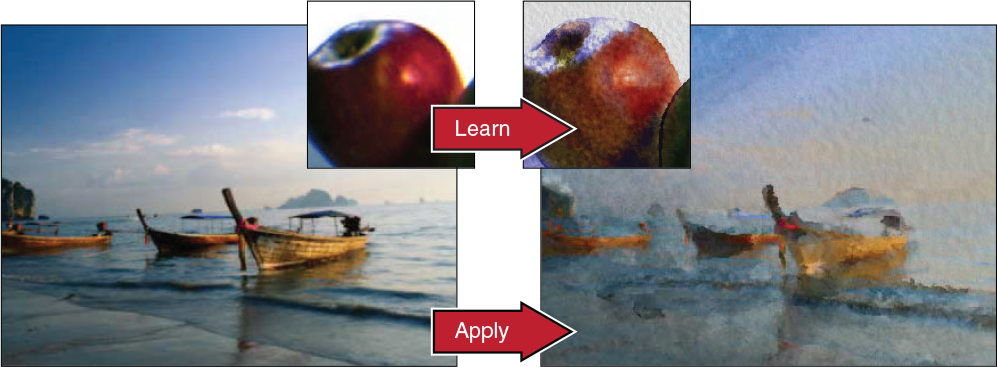
\includegraphics[width=\textwidth]{gfx/style-transfer-analogy}
  \caption{
    The Image Analogies algorithm \cite{Hertzmann2001}.
    Given the apple image and its filtered version, the algorithm learns the luminance transformation that must be applied to the boats image to produce an analogous filtered new image.
  }
  \label{fig:sec:context:style-transfer:style-transfer-analogy}
\end{figure}

Later, in 2003, \citet{Ashikhmin2003} developed an algorithm called Fast Texture Transfer that produces similar results but requires only a single texture sample.
The algorithm uses \emph{Markov random fields} to model the sample texture and then it generates the stylized image by growing texture patches, blending them pixel by pixel with those of the target image.
A limitation of this style transfer approach, also shared with \citeauthor{Hertzmann2001}'s, is that texture coherence can only be preserved locally \cite{Lee2010} and, thus, only small texture patches are applied, as shown in \autoref{fig:sec:context:style-transfer:style-transfer-analogy}.

\begin{figure}[t]
  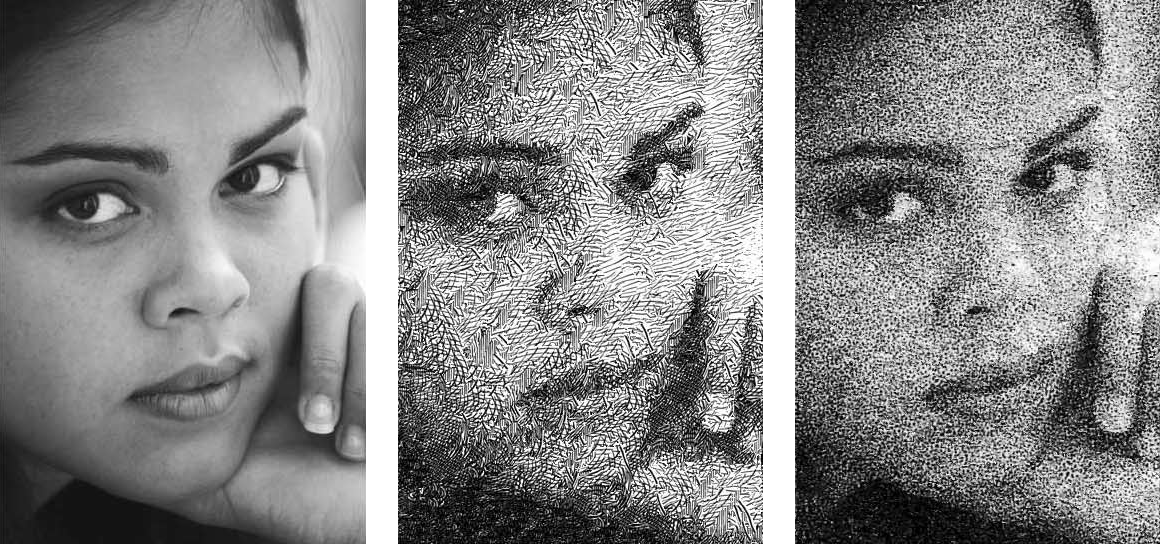
\includegraphics[width=\textwidth]{gfx/style-transfer-fast-texture}
  \caption{
    Results of applying Fast Texture Transfer with different texture samples \cite{Ashikhmin2003}.
    At the left, the target image on which the style is applied.
    At the center, the target image with a hatching drawing texture applied.
    At the right, the target image with a charcoal drawing texture applied.
  }
  \label{fig:sec:context:style-transfer:style-transfer-analogy}
\end{figure}

\citet{Xie2007} proposed in 2007 a new method called Feature Guided Texture Synthesis (FGTS) that better preserves the content of the target image, as we can observe in \autoref{fig:sec:context:style-transfer:style-transfer-feature}.
In this algorithm, first, a feature field is calculated from the target image trying to find edges and corners, assuming those pixels carry more information for the human visual system.
Then, a style transfer process similar to the previous one applies the texture but preserves the pixels specified in the feature field.
This method, like the ones described before, uses low-level statistical features.
\citeauthor{Xie2007} already mentioned the disadvantage of this and anticipated a sharper separation of style and content using higher-level, larger-scale features involving prior human knowledge.

\begin{figure}[t]
  \begin{subfigure}[b]{0.24\textwidth}
    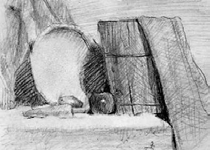
\includegraphics[width=\textwidth]{gfx/style-transfer-feature-1}
    \caption{Style example}
  \end{subfigure}
  \begin{subfigure}[b]{0.24\textwidth}
    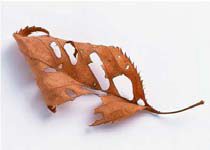
\includegraphics[width=\textwidth]{gfx/style-transfer-feature-2}
    \caption{Target image}
  \end{subfigure}
  \hfill
  \begin{subfigure}[b]{0.24\textwidth}
    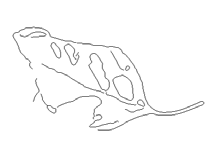
\includegraphics[width=\textwidth]{gfx/style-transfer-feature-3}
    \caption{Feature image}
  \end{subfigure}
  \begin{subfigure}[b]{0.24\textwidth}
    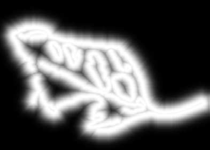
\includegraphics[width=\textwidth]{gfx/style-transfer-feature-4}
    \caption{Feature field}
  \end{subfigure}
  \par\medskip
  \begin{subfigure}[b]{0.5\textwidth}
    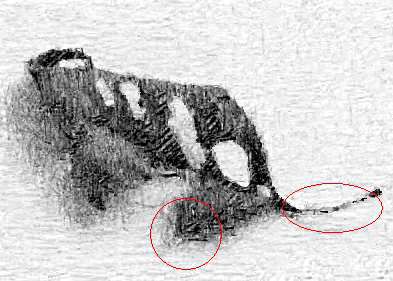
\includegraphics[width=\textwidth]{gfx/style-transfer-feature-5}
    \caption{Analogies}
  \end{subfigure}
  \begin{subfigure}[b]{0.5\textwidth}
    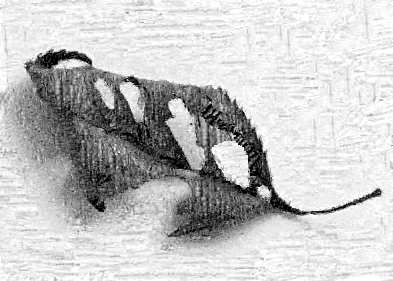
\includegraphics[width=\textwidth]{gfx/style-transfer-feature-6}
    \caption{FGTS}
  \end{subfigure}
  \caption{
    Comparison between Image Analogies and Feature Guided Texture Synthesis \cite{Xie2007}.
    On the top row, from left to right: the style example (a) to be transferred to the target image (b), the computed features from the target image (c), and the feature field defining which pixels carry the most content information and therefore should be preserved (d).
    Bottom left (e), the result produced by image analogy with the most severe content losses highlighted in red.
    Bottom right (f), the result produced by FGTS without the content losses seen in (e).
  }
  \label{fig:sec:context:style-transfer:style-transfer-feature}
\end{figure}

Lastly, in 2010, \citet{Lee2010} proposed an improved method called Directional Texture Transfer that finally transferred larger-scale patterns.
The algorithm attains this goal by taking into account the flow of a target image and interpolating it with that of a style source, using the result as the guide to place brush strokes.
We can see in \autoref{fig:sec:context:style-transfer:style-transfer-directional} how this approach preserves the different regions of the target image very sharply, as the strokes are transferred with different intensity.
This method creates compelling results, but it is limited to stroke-based rendering and far from the generalization we are looking for in a holistic separation of style and content.

\begin{figure}[t]
  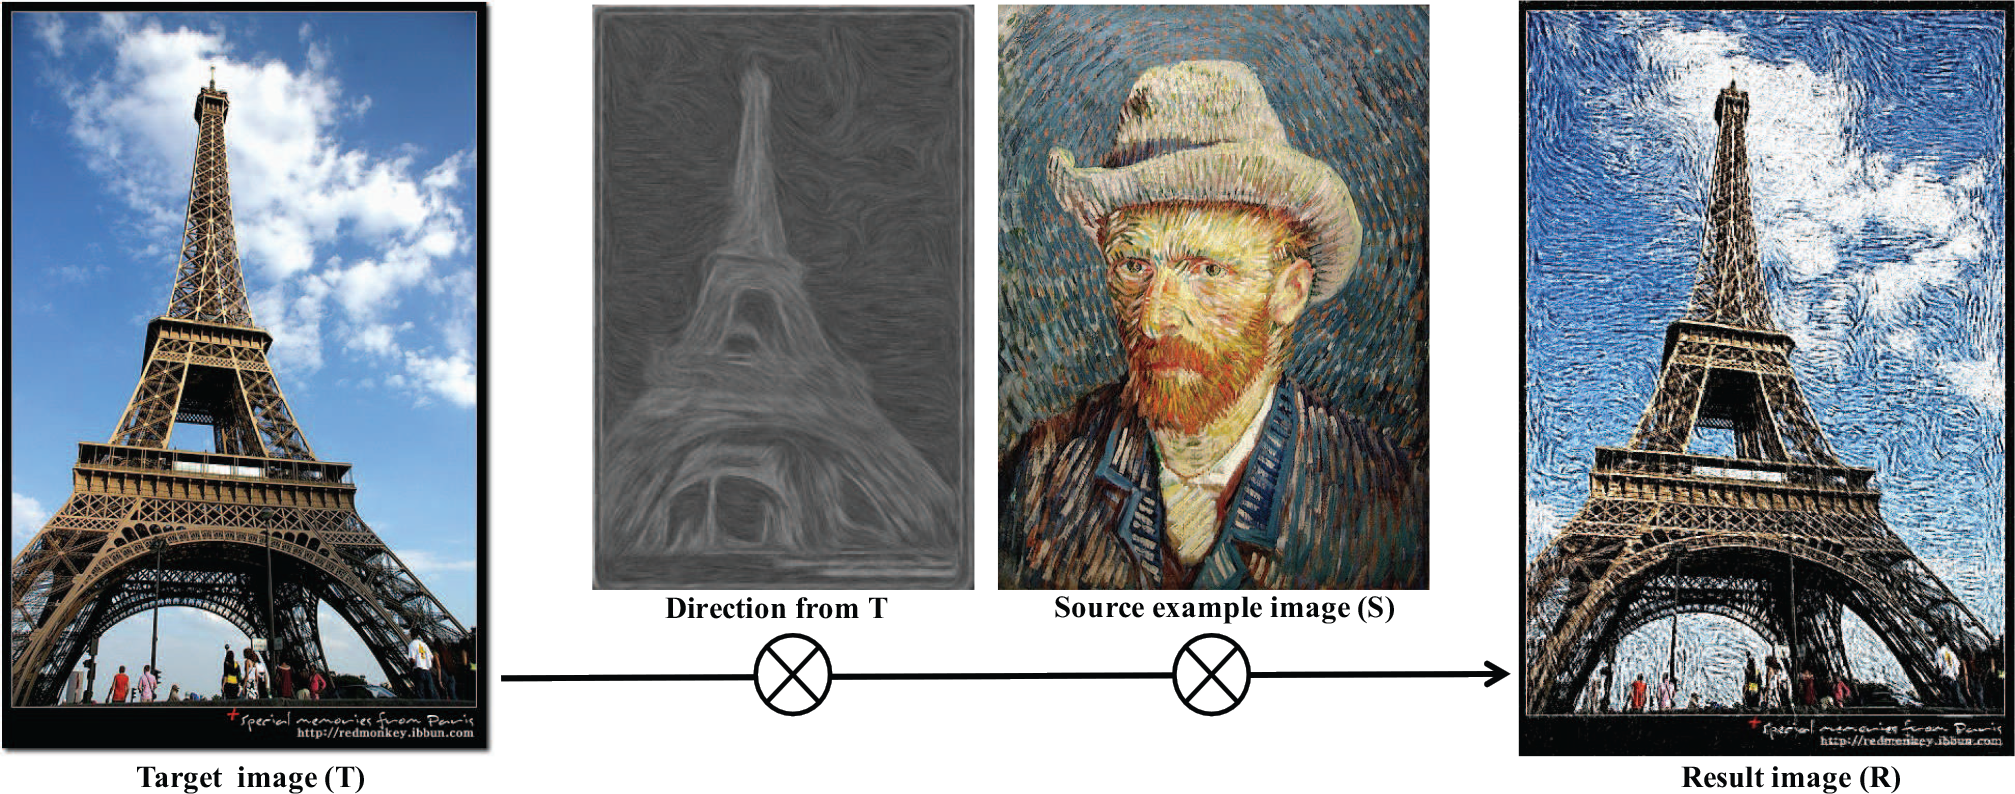
\includegraphics[width=\textwidth]{gfx/style-transfer-directional}
  \caption{
    Results of applying Directional Texture Transfer \cite{Lee2010}.
    First, the flow of the target image (T) is calculated and then interpolated with that of the style source (S), eventually used to guide the strokes that compose the result image (R).
  }
  \label{fig:sec:context:style-transfer:style-transfer-directional}
\end{figure}

\citeauthor{Kyprianidis2013}, in a style transfer techniques survey \cite{Kyprianidis2013} published in 2013, identified a clear tendency towards global-scope approaches, like \citeauthor{Lee2010}'s, rather than to local-level statistical measurements, like the first three ones we discussed in this section.
Global scope approaches require taking larger-scale patterns into account, which is, precisely, what deep neural networks trained for object recognition are very good at.
Two years after \citeauthor{Kyprianidis2013}'s survey, \citeauthor{Gatys2015B}'s Neural Style algorithm \cite{Gatys2015B}, resorted to deep neural networks and outperformed every other technique used in style transfer to date.
Even more interesting, it has given us a way to crack open the problem of separation of style and content.
